% Декомпозиция поверхностной сетки.
\subsection{Декомпозиция поверхностной неструктурированной расчетной сетки}

В этом разделе будем рассматривать подходы к декомпозиции неструктурированной поверхностной расчетной сетки с треугольными ячейками\label{term:unstruct_surf_calc_mesh3} \cite{Rybakov2020Decomp}.
В отличие от блочно-структурированных сеток\label{term:mesh_block_struct4} у рассматриваемой неструктурированной сетки ячейки не объединяются в блоки, а являются независимыми объектами проведения расчетов.
Для неструктурированных поверхностных сеток будем считать, что вычислительная окрестность\label{term:cell_calc_template2} каждой ячейки будет влючать кроме нее самом только три смежные ячейки (граничащие с рассматривамой по каждому из трех ребер).

\subsubsection{Описание методов декомпозиции}

Будем рассматривать алгоритмы декомпозиции на примере тестовой трехмерной поверхностной сетки (wing), состоящей из ячеек-треугольников.
Сетка представляет собой профиль крыла летательного аппарата и содержит порядка $n = 2 \cdot 10^4$ ячеек.
Внешний вид тестовой расчетной сетки представлен на рис.~\ref{fig:text_2_decompsurf_wing_grid}.
Этот трехмерный профиль был сгенерирован из двумерного профиля NACA 0012.

\begin{figure}[ht]
\centering
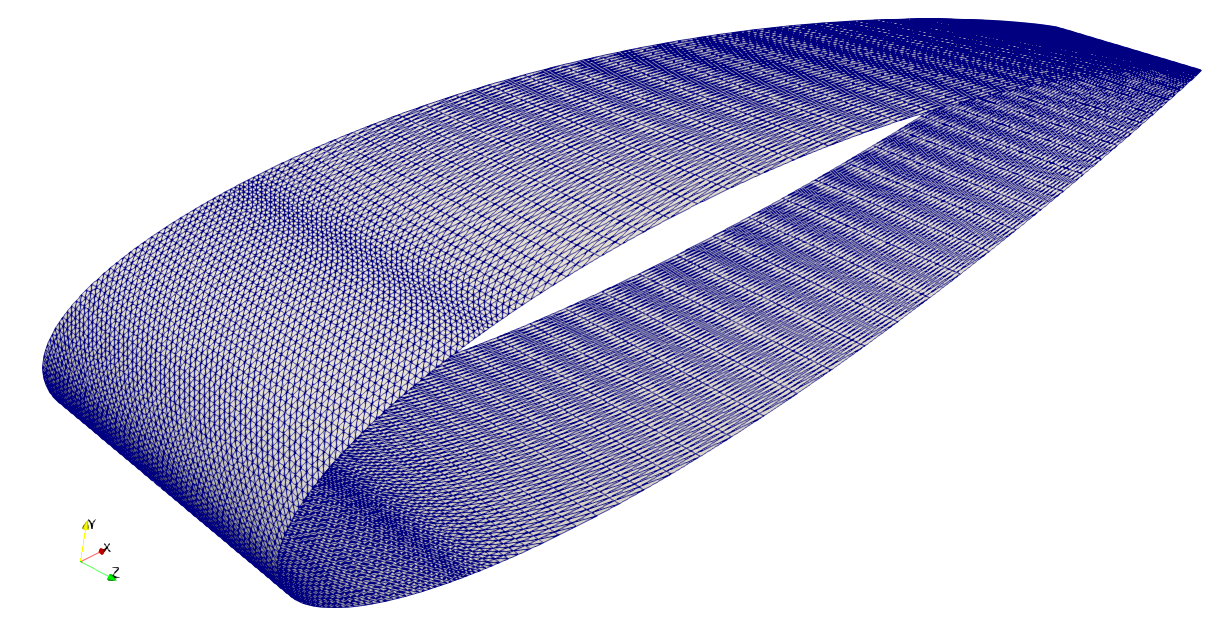
\includegraphics[width=0.5\textwidth]{./pics/text_2_decompsurf/wing_grid.png}
\singlespacing
\captionstyle{center}\caption{Внешний вид расчетной сетки wing, используемой для тестирования алгоритмов декомпозиции.}
\label{fig:text_2_decompsurf_wing_grid}
\end{figure}

\begin{figure}[ht]
\centering
\begin{tabular}{ll}
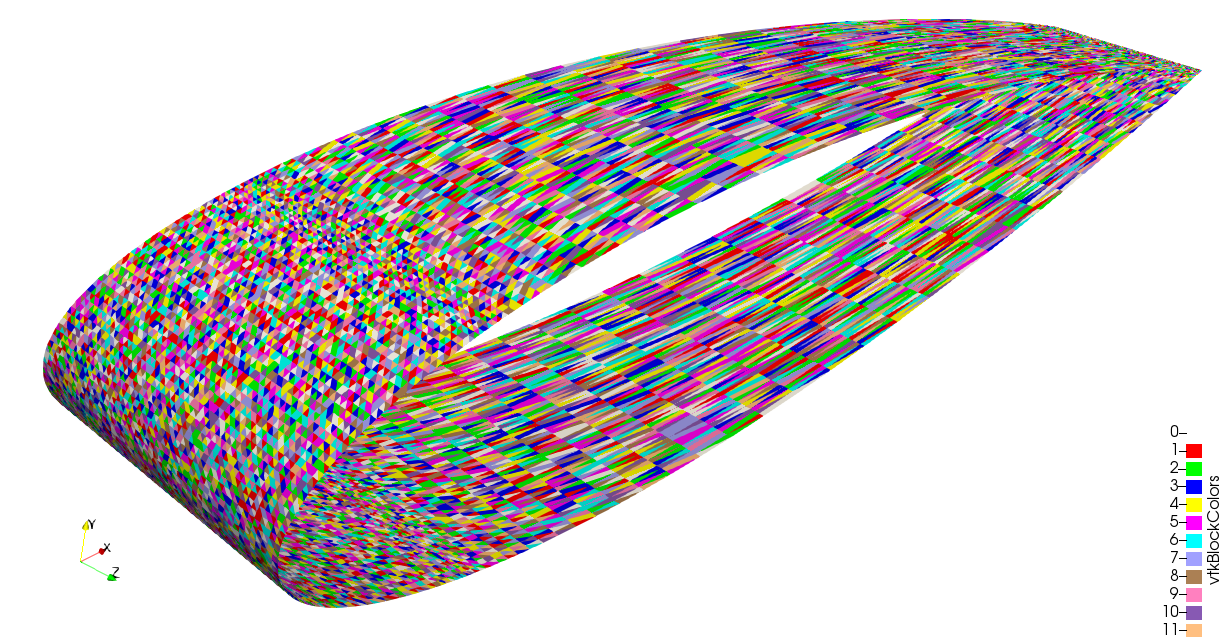
\includegraphics[width=0.45\textwidth]{./pics/text_2_decompsurf/wing_random_32.png}
&
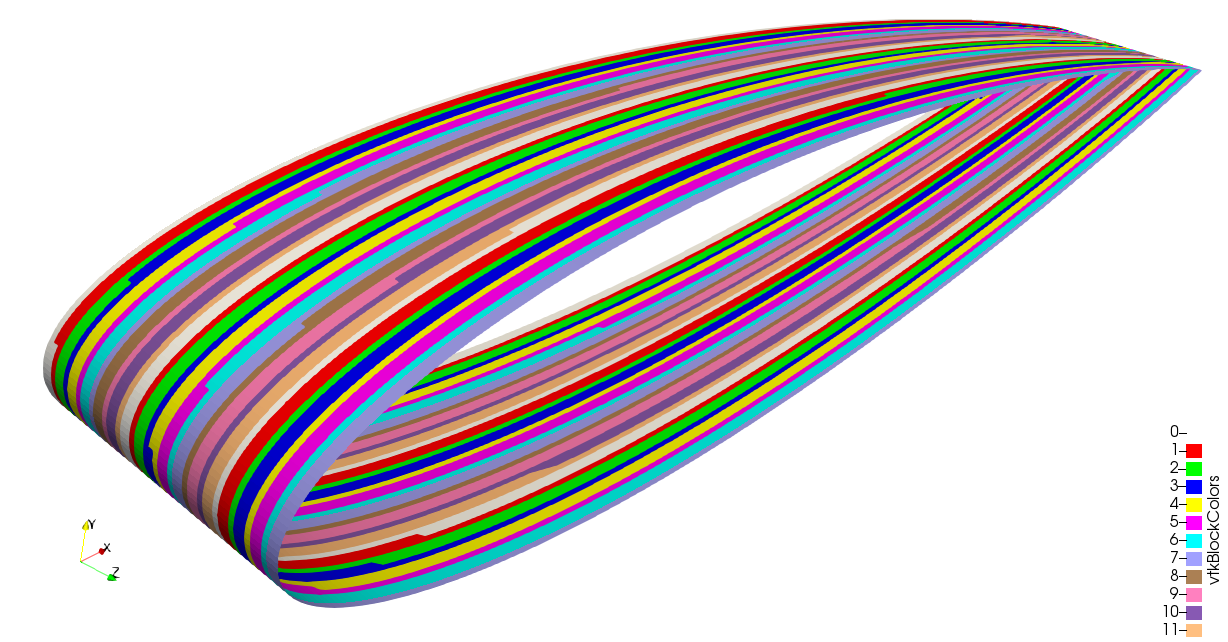
\includegraphics[width=0.45\textwidth]{./pics/text_2_decompsurf/wing_linear_32.png}
\\
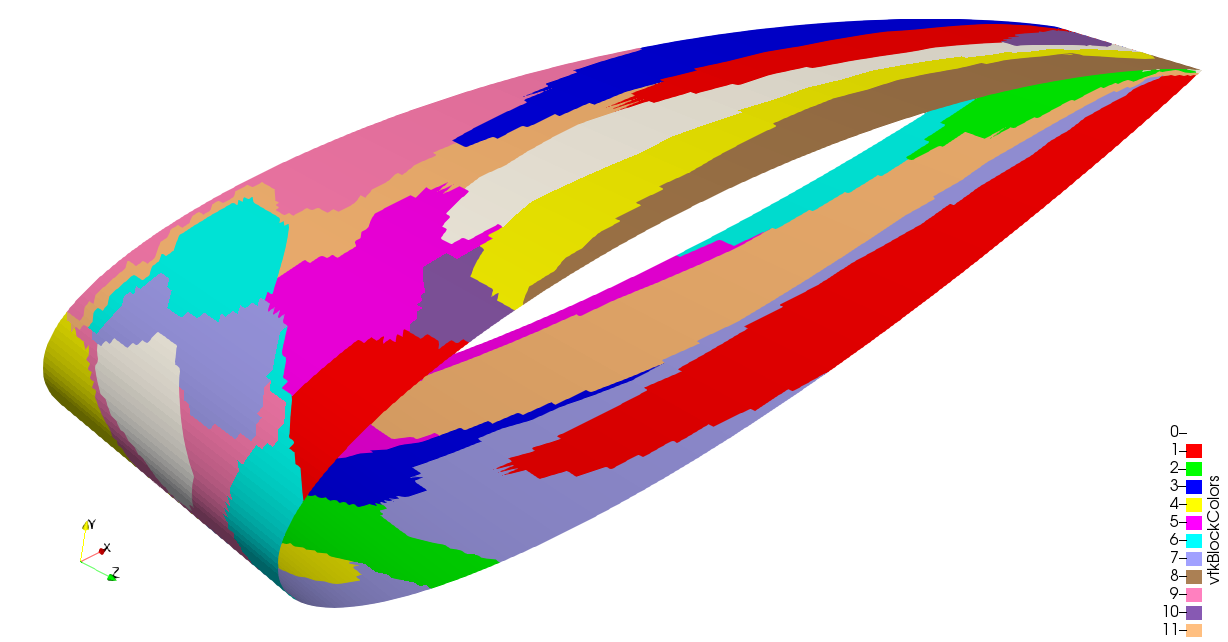
\includegraphics[width=0.45\textwidth]{./pics/text_2_decompsurf/wing_rgrow_32.png}
&
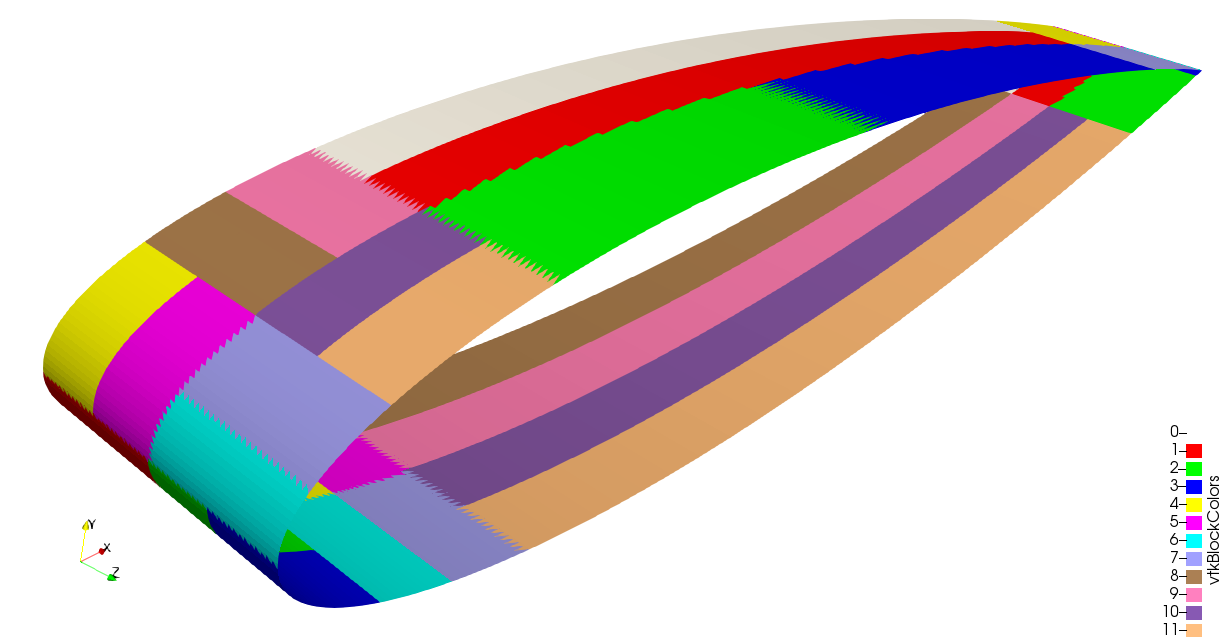
\includegraphics[width=0.45\textwidth]{./pics/text_2_decompsurf/wing_hierarchical_32.png}
\end{tabular}
\singlespacing
\captionstyle{center}\caption{Результат декомпозиции расчетной сетки на 32 домена. Сверху вниз слева направо -- случайное распределение, линейное распределение, наращивание доменов и иерархическое дробление\label{term:alg_decomp_hierarch}.}
\label{fig:text_2_decompsurf_4}
\end{figure}

В качестве первого и самого простого алгоритма декомпозиции рассмотрим алгоритм случайного распределения\label{term:alg_decomp_random} ячеек расчетной сетки по доменам.
Результат применения этого алгоритма к тестовой сетке показан на рис.~\ref{fig:text_2_decompsurf_4} сверху слева.
Алгоритм случайного распределения имеет достаточно низкое значение по критерию $D$\label{term:decomp_neravn3}, то есть распределение ячеек по доменам равномерное, однако при случайном распределении практически все ребра с высокой долей вероятности являются междоменными\label{term:edge_cross2}, что порождает огромный объем данных, которыми нужно обмениваться при синхронизации вычислений.
Также следует отменить, что при случайном распределении ячеек по доменам любые два домена\label{term:domain2} оказываются соседними, граф связности доменов является полным.
Таким образом, каждый домен должен обмениваться данными со всеми остальными доменами по достаточно протяженным границам.
Также алгоритм становится совершенно непригодным, когда возникает необходимость создания теневых слоев\label{term:block_shadow_layer2} глубиной больше единицы.
Использование таких буферных зон может потребоваться для реализации численных методов повышенной точности.

\begin{figure}[ht]
\centering
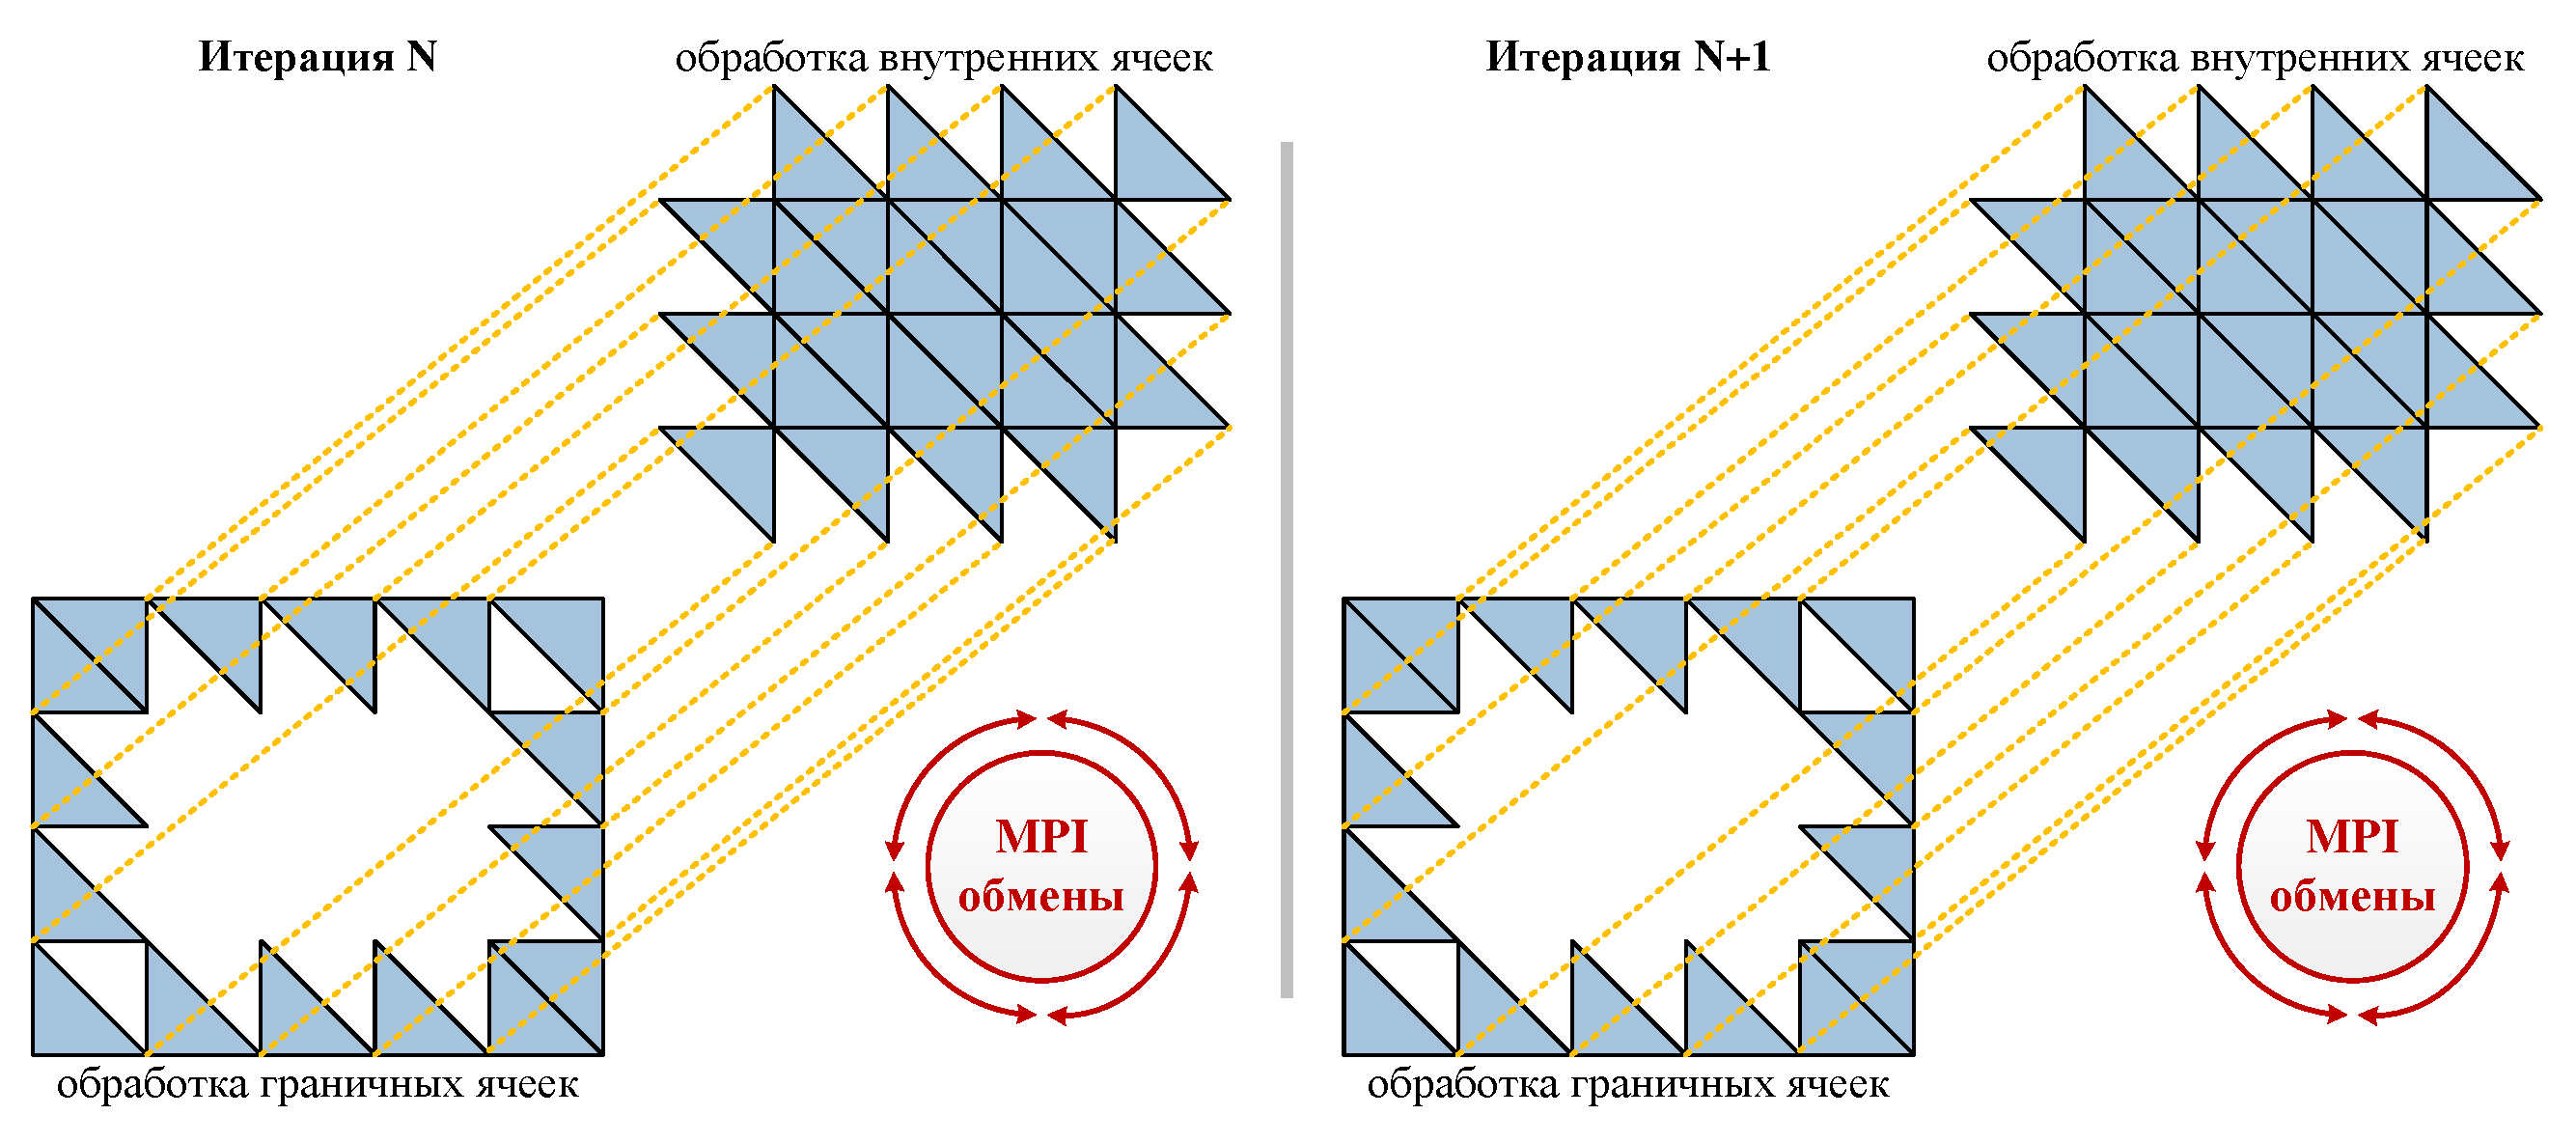
\includegraphics[width=0.8\textwidth]{./pics/text_2_decompsurf/mpi_border_inner.pdf}
\singlespacing
\captionstyle{center}\caption{Сокрытие издержек на информационные обмены за вычислениями.}
\label{fig:text_2_decompsurf_wing_border_inner}
\end{figure}

На этом этапе упомянем механизм частичного сокрытия издержек на обмены данными за основными вычислениями.
Все ячейки каждого домена можно разделить на внутренние\label{term:cell_block_inner2} и граничные\label{term:cell_block_border2} (аналогично внутренним и граничным ячейкам блока для блочно-структурированных сеток).
Ценность внутренних ячеек состоит в том, что они не участвуют в обменах данными с соседними доменами, поэтому обработку внутренних ячеек на следующей итерации расчетов можно начинать, не дожидаясь завершения обменов данными на ребрах, составляющих границу между доменами (см. рис.~\ref{fig:text_2_decompsurf_wing_border_inner}).
Понятно, что такой подход неприменим при использовании случайного распределения ячеек по доменам, так как в большинстве случаев множества внутренних ячеек доменов оказываются практически пустыми.

Рассмотрим семейство алгоритмов декомпозиции, в которых учитываются только индексы распределяемых ячеек и никак не учитываются другие их данные.
Под индексом в данном случае понимается номер ячейки в общем массиве ячеек расчетной сетки.
Уже по этому факту становится понятно, что такие алгоритмы не могут претендовать на высокое качество, так как их результат существенным образом зависит просто от порядка хранения данных расчетной сетки.
Самым простым из алгоритмов этого класса является алгоритм линейного распределения ячеек\label{term:alg_decomp_linear} по доменам.
Так как в каждый домен в среднем должно войти по $\frac{n}{k}$ ячеек (для простоты не будем обращать внимание на то, что это число может быть нецелым), то можно ячейки с номерами из диапазона $[0, \frac{n}{k} - 1]$ отнести к первому домену, ячейки с номерами $[\frac{n}{k}, \frac{2n}{k} - 1]$ ко второму домену и так далее.
При такой декомпозиции, конечно, можно добиться равномерного распределения ячеек по доменам, однако значения параметров $L$\label{term:decomp_maxbord2} и $I$\label{term:decomp_sumbord2} в общем случае предугадать невозможно.
Например, на рассматриваемой тестовой сетке видно, что деление на домены вдоль профиля крыла (как это показано на рис.~\ref{fig:text_2_decompsurf_4} сверху справа) порождает очень длинные границы между соседними доменами.
Было бы гораздо эффективнее производить деление сетки поперек профиля.

В общем случае ячейки с непрерывным диапазоном индексов не обязаны составлять не то что компактные домены с границами небольшой протяженности, а вообще могут порождать несвязные домены, с артефактами, выколотыми ячейками и так далее.
Применение таких алгоритмов оправдано только при обладании некоторой априорной информацией о структуре расчетной сетки (например, если известно, что сетка на самом деле является блочно-структурированной, в которой отдельные блоки соответствуют непрерывным диапазонам индексов ячеек).

Большой класс алгоритмов формируется из так называемых алгоритмов наращивания доменов\label{term:alg_decomp_rgrow}.
В основе этих алгоритмов лежит следующий принцип: вначале выбирается ячейка (или несколько ячеек), от которой далее производится наращивание домена путем последовательного добавления к ней соседних ячеек.
В рамках этого класса алгоритмов при последовательном создании доменов размера $\frac{n}{k}$ получим жадный алгоритм Фархата\label{term:alg_decomp_farhat}, результатом которого являются домены с очень протяженными границами \cite{Farhat1988Decomp}.
При использовании одновременного роста сразу нескольких доменов от случайных ячеек расчетной сетки получаем алгоритм пузырькового роста \cite{Preis1997Decomp}\label{term:alg_decomp_bubble}, который требуется запускать на расчетной сетке итерационно несколько раз для получения приемлемых характеристик качества разбиения.
При этом алгоритм пузырькового роста не гарантирует сбалансированного разбиения ячеек сетки по доменам (для достижения этого необходимо производить дополнительную коррекцию).
Также следует отметить инкрементальный алгоритм декомпозиции графов \cite{Yakobovsky2005Decomp}\label{term:alg_decomp_inc}, особенностью которого является возможность освобождения части ячеек, уже распределенных по доменам, с последующим повторением роста доменов.

Мы рассматриваем простой алгоритм наращивания доменов, в котором все домены наращиваются одновременно, начиная с некоторых случайно выбранных ячеек сетки.
При этом поддерживается связность доменов -- если в какой-то момент домену больше некуда расти, то он прекращает свое наращивание и больше не расширяется.
Таким образом, возможно генерация крайне неравномерных по количеству ячеек доменов. Пример результата применения описанного алгоритма приведен на рис.~\ref{fig:text_2_decompsurf_4} снизу слева.

Кроме приведенных алгоритмов существует еще большое количество подходов к декомпозиции расчетных сеток, среди них алгоритмы, основанные на методе спектральной бисекции \cite{Urschel2014Decomp}, диффузионные и генетические алгоритмы \cite{Zhao2019Decomp}, иерархические алгоритмы \cite{Kapyris1998Decomp} и многие другие.
Наиболее полный обзор различных алгоритмов декомпозиции расчетных сеток можно найти в \cite{Golovchenko2020Decomp} и \cite{Zheleznyakova2017Decomp}.

\subsubsection{Алгоритм декомпозиции с помощью иерархического \\ дробления}\label{sec:text_2_decompsurf_hierarchical}

\label{term:alg_decomp_inc}В работе \cite{Golovchenko2020Decomp} описан параллельный алгоритм геометрической декомпозиции сеточных данных.
Во время работы этого алгоритма происходит последовательное деление текущего домена пополам с помощью сечения плоскостью.
На рис.~\ref{fig:text_2_decompsurf_hierarchical} продемонстрирована схема, по которой изначальный головной домен h делится на пару доменов hl (left), hr (right), каждый из которых делится далее пополам и так далее на любое количество доменов, равное степени двойки.

\begin{figure}[ht]
\centering
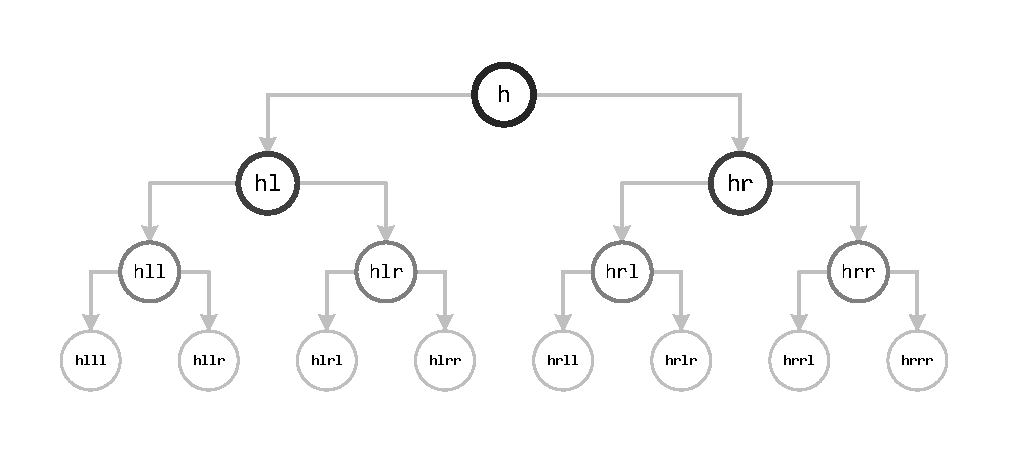
\includegraphics[width=0.6\textwidth]{./pics/text_2_decompsurf/hierarchical.pdf}
\singlespacing
\captionstyle{center}\caption{Иллюстрация иерархического трехуровневого разделения головного домена.}
\label{fig:text_2_decompsurf_hierarchical}
\end{figure}

Этот алгоритм предлагается расширить, введя в него произвольные критерии разбиения текущего домена на пару более мелких доменов.
Вначале рассмотрим схему простого деления домена пополам с использованием произвольного признака, по которому производится деление (см. рис.~\ref{fig:text_2_decompsurf_split}).

\begin{figure}[ht]
\centering
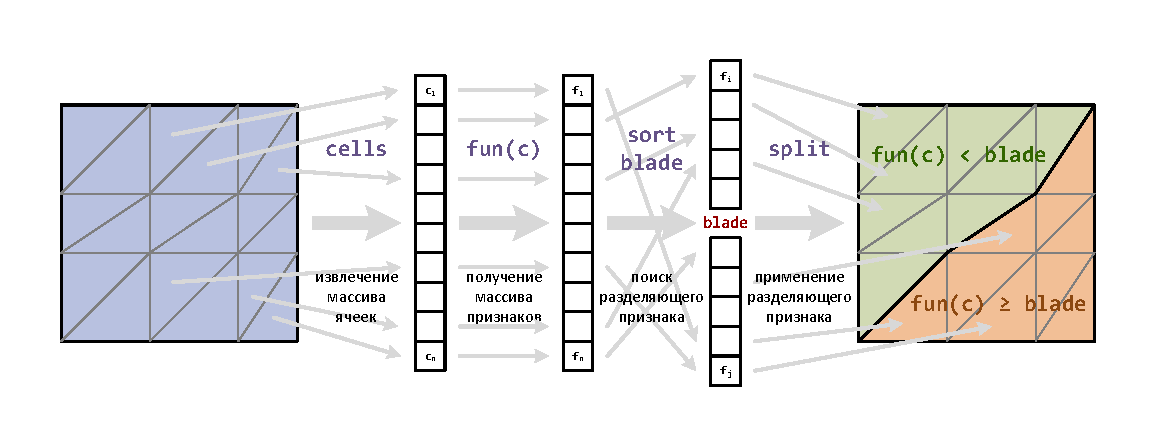
\includegraphics[width=0.9\textwidth]{./pics/text_2_decompsurf/split.pdf}
\singlespacing
\captionstyle{center}\caption{Схема выполнения разделения домена пополам по заданному признаку fun.}
\label{fig:text_2_decompsurf_split}
\end{figure}

Пусть задан массив ячеек домена $C$ и произвольная функция извлечения признака из ячейки $fun$.
Первым шагом является вычисление массива признаков для всех ячеек.
После этого половина массива с меньшими значениями признака формирует один дочерний домен, а вторая половина с большими значениями признакак формирует второй дочерний домен.

После разделения домена на два более мелких домена можно вычислить параметр, отражающий эффективность разбиения.
В качестве такого параметра предлагается использовать длину границы между двумя образованными новыми доменами.
Таким образом, критерий разбиения зависит от функции вычисления признака $fun$.
В свою очередь это означает, что при выполнении разбиения не обязательно ограничиваться одной функцией вычисления признака, вместо этого можно подать список функций, для каждой функции вычислитель показатель качества разбиения и в результате остановиться на той функции вычисления признака, которая в конечном итоге приводит к наиболее эффективному разбиению.
Если в качестве функций вычисления признака ячейки использовать просто извлечение трех координат центров ячеек, то мы получим в чистом виде алгоритм геометрической декомпозиции сетки с выбором для дробления наиболее протяженного размера по одной из координат.
Результат применения этого алгоритма показан на рис.~\ref{fig:text_2_decompsurf_4} снизу справа.

Варьируя набор функций вычисления признаков, по которым можно выполнять разбиение домена, возможно выполнять геометрическую декомпозицию вдоль направления любой кривой, для которой вычисляется проекция ячейки.
Декомпозиция с помощью данного метода не ограничивается только геометрическими признаками.
Функции вычисления признаков могут использоваться для анализа физических данных ячеек, например, для локализации и выделении в отдельные домены областей с повышенным давлением.

\subsubsection{Результаты экспериментов по декомпозиции расчетных \\ сеток на профиле крыла}

\begin{figure}[H]
\centering
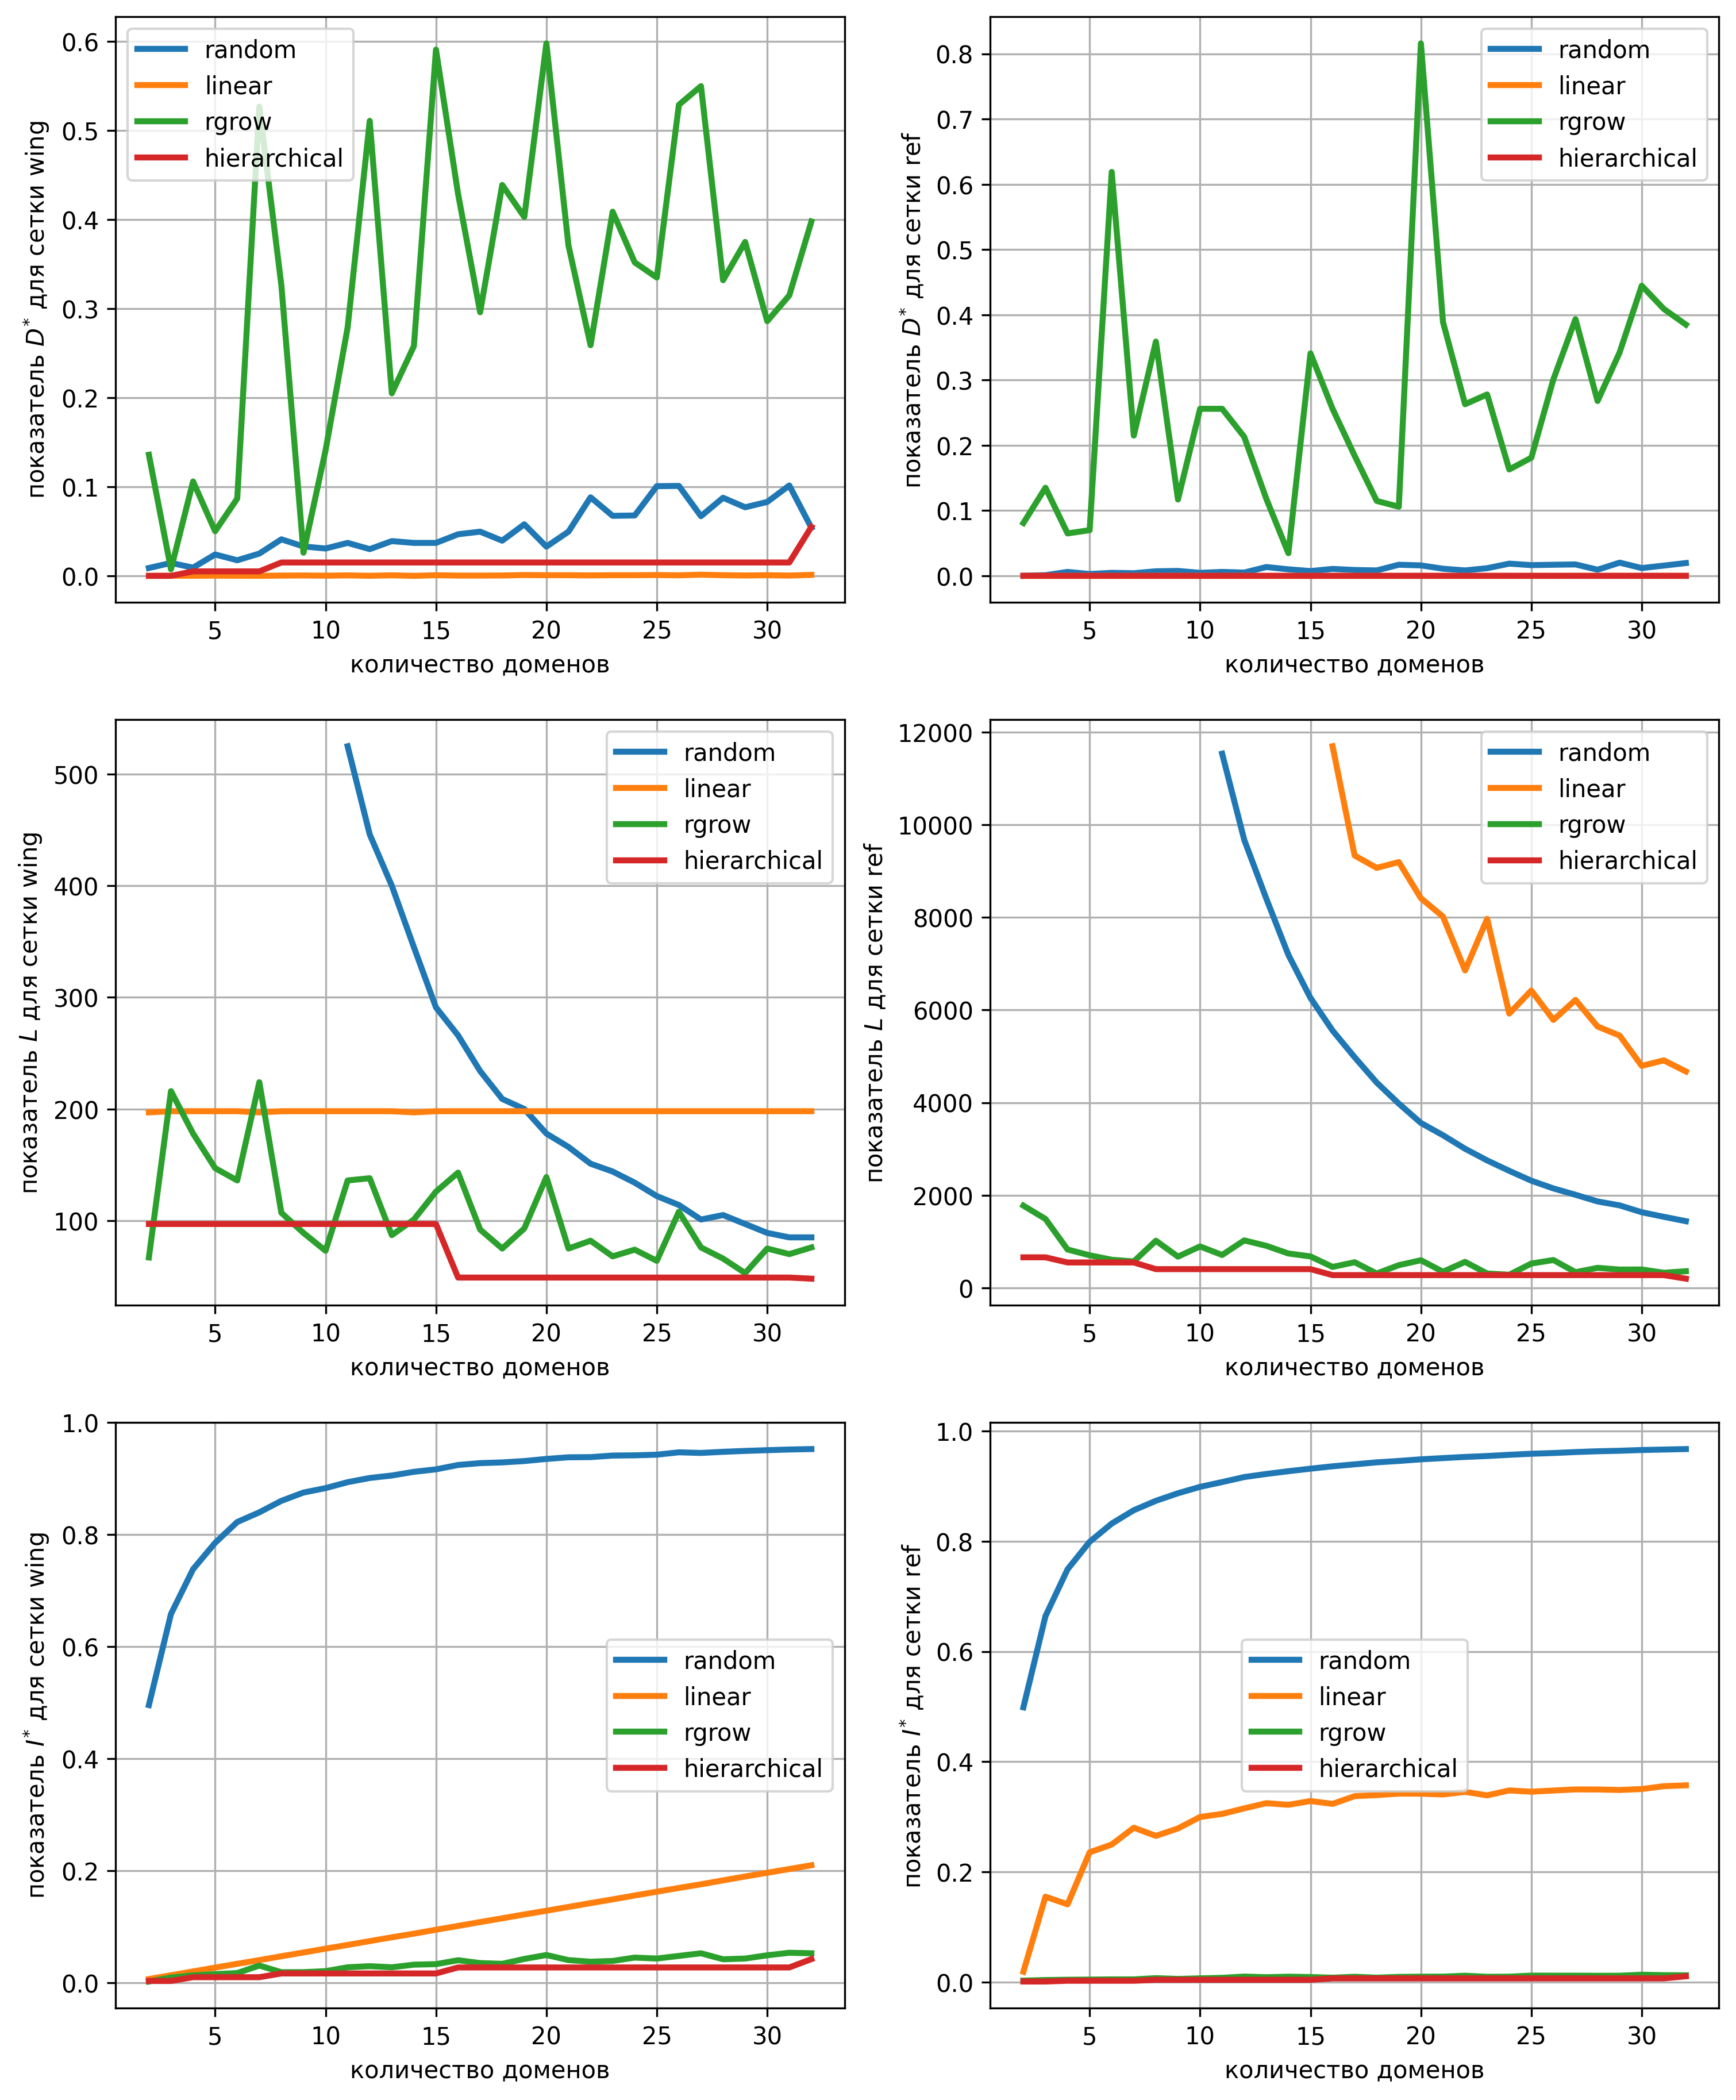
\includegraphics[width=1.0\textwidth]{./pics/text_2_decompsurf/qual.png}
\singlespacing
\captionstyle{center}\caption{Графики показателей $D^{*}$, $L$, $I^{*}$ для сеток wing и ref.}
\label{fig:text_2_decompsurf_qual}
\end{figure}

На рис.~\ref{fig:text_2_decompsurf_qual} представлены графики параметров $D^{*}$, $L$, $I^{*}$, вычисленные во время применения различных алгоритмов декомпозиции поверхностной расчетной сетки на разное количество доменов от 2 до 32.

Для эксперимента использовались две сетки.
Первая сетка -- wing, представленная на рис.~\ref{fig:text_2_decompsurf_wing_grid}.
Вторая сетка -- ref -- более приближена к реальной геометрии летательного аппарата и содержит порядка $n = 4 \cdot 10^5$ ячеек.
На графиках введены следующие краткие названия алгоритмов: random -- случайное распределение ячеек по доменам\label{term:alg_decomp_random2}, linear -- линейное разделение ячеек между доменами по индексу\label{term:alg_decomp_linear2}, rgrow -- алгоритм наращивания доменов от случайных ячеек\label{term:alg_decomp_rgrow2}, hierarchical -- иерархическое дробление доменов\label{term:alg_decomp_hierarch2} пополам по одной из трех координат (в качестве функций вычисления признаков ячеек брались просто функции извлечения каждой из трех координат центра ячейки).

При этом отметим, что при использовании алгоритма rgrow умышленно использовалась только одна итерации наращивания, для демонстрации того, насколько неравномерным может быть распределение размеров доменов при случайном выборе инициирующих ячеек (из рисунков видно, что значение параметра $D^{*}$\label{term:decomp_neravn4} достигает значениий 0,6 и 0,8 для сеток wing и ref соответственно).

Из приведенных графиков можно сделать выводы, что из представленных алгоритмов иерархическое деление доменов с выбором оптимального критерия деления из списка функций вычисления признаков ячеек является наиболее приемлемым по параметрам $D^{*}$, $L$,\label{term:decomp_maxbord3} $I^{*}$,\label{term:decomp_sumbord3} то есть с помощью этого алгоритма генерируется достаточно равномерное распределение ячеек по доменам при низкой общей доле междоменных ребер и малой протяженности границ между доменами.
